%% BioMed_Central_Tex_Template_v1.06
%%                                      %
%  bmc_article.tex            ver: 1.06 %
%                                       %

%%IMPORTANT: do not delete the first line of this template
%%It must be present to enable the BMC Submission system to
%%recognise this template!!

%%%%%%%%%%%%%%%%%%%%%%%%%%%%%%%%%%%%%%%%%
%%                                     %%
%%  LaTeX template for BioMed Central  %%
%%     journal article submissions     %%
%%                                     %%
%%          <8 June 2012>              %%
%%                                     %%
%%                                     %%
%%%%%%%%%%%%%%%%%%%%%%%%%%%%%%%%%%%%%%%%%


%%%%%%%%%%%%%%%%%%%%%%%%%%%%%%%%%%%%%%%%%%%%%%%%%%%%%%%%%%%%%%%%%%%%%
%%                                                                 %%
%% For instructions on how to fill out this Tex template           %%
%% document please refer to Readme.html and the instructions for   %%
%% authors page on the biomed central website                      %%
%% http://www.biomedcentral.com/info/authors/                      %%
%%                                                                 %%
%% Please do not use \input{...} to include other tex files.       %%
%% Submit your LaTeX manuscript as one .tex document.              %%
%%                                                                 %%
%% All additional figures and files should be attached             %%
%% separately and not embedded in the \TeX\ document itself.       %%
%%                                                                 %%
%% BioMed Central currently use the MikTex distribution of         %%
%% TeX for Windows) of TeX and LaTeX.  This is available from      %%
%% http://www.miktex.org                                           %%
%%                                                                 %%
%%%%%%%%%%%%%%%%%%%%%%%%%%%%%%%%%%%%%%%%%%%%%%%%%%%%%%%%%%%%%%%%%%%%%

%%% additional documentclass options:
%  [doublespacing]
%  [linenumbers]   - put the line numbers on margins

%%% loading packages, author definitions

%\documentclass[twocolumn]{bmcart}% uncomment this for twocolumn layout and comment line below
\documentclass{bmcart}

%%% Load packages
%\usepackage{amsthm,amsmath}
%\RequirePackage{natbib}
\RequirePackage{hyperref}
\usepackage[utf8]{inputenc} %unicode support
%\usepackage[applemac]{inputenc} %applemac support if unicode package fails
%\usepackage[latin1]{inputenc} %UNIX support if unicode package fails


%%%%%%%%%%%%%%%%%%%%%%%%%%%%%%%%%%%%%%%%%%%%%%%%%
%%                                             %%
%%  If you wish to display your graphics for   %%
%%  your own use using includegraphic or       %%
%%  includegraphics, then comment out the      %%
%%  following two lines of code.               %%
%%  NB: These line *must* be included when     %%
%%  submitting to BMC.                         %%
%%  All figure files must be submitted as      %%
%%  separate graphics through the BMC          %%
%%  submission process, not included in the    %%
%%  submitted article.                         %%
%%                                             %%
%%%%%%%%%%%%%%%%%%%%%%%%%%%%%%%%%%%%%%%%%%%%%%%%%


%\def\includegraphic{}
%\def\includegraphics{}



%%% Put your definitions there:
\startlocaldefs
\setlength{\marginparwidth}{2cm}
%\usepackage[disable]{todonotes}
\usepackage[draft]{todonotes}
\endlocaldefs


%%% Begin ...
\begin{document}

%%% Start of article front matter
\begin{frontmatter}

\begin{fmbox}
\dochead{Data Note}

%%%%%%%%%%%%%%%%%%%%%%%%%%%%%%%%%%%%%%%%%%%%%%
%%                                          %%
%% Enter the title of your article here     %%
%%                                          %%
%%%%%%%%%%%%%%%%%%%%%%%%%%%%%%%%%%%%%%%%%%%%%%

\title{Deeply sequenced metagenome and metatranscriptome of a biogas-producing microbial community from an agricultural production-scale biogas plant}

%%%%%%%%%%%%%%%%%%%%%%%%%%%%%%%%%%%%%%%%%%%%%%
%%                                          %%
%% Enter the authors here                   %%
%%                                          %%
%% Specify information, if available,       %%
%% in the form:                             %%
%%   <key>={<id1>,<id2>}                    %%
%%   <key>=                                 %%
%% Comment or delete the keys which are     %%
%% not used. Repeat \author command as much %%
%% as required.                             %%
%%                                          %%
%%%%%%%%%%%%%%%%%%%%%%%%%%%%%%%%%%%%%%%%%%%%%%

\author[
   addressref={cebitec,techfak},
%   corref={cebitec},
   email={abremges@cebitec.uni-bielefeld.de}
]{\inits{AB}\fnm{Andreas} \snm{Bremges}}
\author[
   addressref={cebitec}
]{\inits{IM}\fnm{Irena} \snm{Maus}}
\author[
   addressref={techfak}
]{\inits{PB}\fnm{Peter} \snm{Belmann}}
\author[
   addressref={cebitec}
]{\inits{FE}\fnm{Felix} \snm{Eikmeyer}}
\author[
   addressref={cebitec}
]{\inits{AW}\fnm{Anika} \snm{Winkler}}
\author[
   addressref={cebitec}
]{\inits{AA}\fnm{Andreas} \snm{Albersmeier}}
\author[
   addressref={cebitec}
]{\inits{AP}\fnm{Alfred} \snm{Pühler}}
\author[
   addressref={cebitec},
   noteref={n1}
]{\inits{ASch}\fnm{Andreas} \snm{Schlüter}}
\author[
   addressref={cebitec,techfak},
   corref={cebitec},
   noteref={n1},
   email={asczyrba@cebitec.uni-bielefeld.de}
]{\inits{AScz}\fnm{Alexander} \snm{Sczyrba}}

%%%%%%%%%%%%%%%%%%%%%%%%%%%%%%%%%%%%%%%%%%%%%%
%%                                          %%
%% Enter the authors' addresses here        %%
%%                                          %%
%% Repeat \address commands as much as      %%
%% required.                                %%
%%                                          %%
%%%%%%%%%%%%%%%%%%%%%%%%%%%%%%%%%%%%%%%%%%%%%%

\address[id=cebitec]{%                           % unique id
  \orgname{Center for Biotechnology, Bielefeld University}, % university, etc
  %\street{Universitätsstraße 27},                     %
  \postcode{33615}                                % post or zip code
  \city{Bielefeld},                              % city
  \cny{Germany}                                    % country
}
\address[id=techfak]{%
  \orgname{Faculty of Technology, Bielefeld University},
  %\street{Universitätsstraße 25},
  \postcode{33615}
  \city{Bielefeld},
  \cny{Germany}
}

%%%%%%%%%%%%%%%%%%%%%%%%%%%%%%%%%%%%%%%%%%%%%%
%%                                          %%
%% Enter short notes here                   %%
%%                                          %%
%% Short notes will be after addresses      %%
%% on first page.                           %%
%%                                          %%
%%%%%%%%%%%%%%%%%%%%%%%%%%%%%%%%%%%%%%%%%%%%%%

\begin{artnotes}
%\note{Sample of title note}     % note to the article
\note[id=n1]{Equal contributor} % note, connected to author
\end{artnotes}

\end{fmbox}% comment this for two column layout

%%%%%%%%%%%%%%%%%%%%%%%%%%%%%%%%%%%%%%%%%%%%%%
%%                                          %%
%% The Abstract begins here                 %%
%%                                          %%
%% Please refer to the Instructions for     %%
%% authors on http://www.biomedcentral.com  %%
%% and include the section headings         %%
%% accordingly for your article type.       %%
%%                                          %%
%%%%%%%%%%%%%%%%%%%%%%%%%%%%%%%%%%%%%%%%%%%%%%

\begin{abstractbox}

\begin{abstract} % abstract
\parttitle{Background}
The production of biogas takes place under anaerobic conditions and involves microbial decomposition of organic matter, with most participating microbes still considered unknown and non-cultivable. Accordingly, metagenome sequencing is currently the only possibility to obtain insights into community composition and the genetic repertoire.
%a presentation of the interest or relevance of these data for the broader community
%
\parttitle{Findings}
Here, we report the first deeply sequenced metagenome and metatranscriptome of a complex biogas-producing microbial community from an agricultural production-scale biogas plant. We assembled the metagenome and reconstructed most genes involved in the methane metabolism, a key pathway involving methanogenesis populated by low-abundance archaea. This exemplary result indicates sufficient sequencing coverage for most downstream analyses.
%a very brief preview of the data type(s) produced, the methods used, and information relevant to data validation
%
\parttitle{Conclusions}
Sequenced at least one order of magnitude deeper than previous studies, our metagenome data will enable novel insights into community composition and the genetic potential of important community members. Moreover, mapping of transcripts to reconstructed genome sequences will enable the identification of active metabolic pathways in target organisms.
%a short summary of the potential uses of these data and implications for the field
\end{abstract}

%%%%%%%%%%%%%%%%%%%%%%%%%%%%%%%%%%%%%%%%%%%%%%
%%                                          %%
%% The keywords begin here                  %%
%%                                          %%
%% Put each keyword in separate \kwd{}.     %%
%%                                          %%
%%%%%%%%%%%%%%%%%%%%%%%%%%%%%%%%%%%%%%%%%%%%%%

\begin{keyword}
\kwd{Biogas}
\kwd{Metagenome}
\kwd{Metatranscriptome}
\kwd{Sequencing}
\kwd{Assembly}
\end{keyword}

% MSC classifications codes, if any
%\begin{keyword}[class=AMS]
%\kwd[Primary ]{}
%\kwd{}
%\kwd[; secondary ]{}
%\end{keyword}

\end{abstractbox}
%
%\end{fmbox}% uncomment this for twcolumn layout

\end{frontmatter}

%%%%%%%%%%%%%%%%%%%%%%%%%%%%%%%%%%%%%%%%%%%%%%
%%                                          %%
%% The Main Body begins here                %%
%%                                          %%
%% Please refer to the instructions for     %%
%% authors on:                              %%
%% http://www.biomedcentral.com/info/authors%%
%% and include the section headings         %%
%% accordingly for your article type.       %%
%%                                          %%
%% See the Results and Discussion section   %%
%% for details on how to create sub-sections%%
%%                                          %%
%% use \cite{...} to cite references        %%
%%  \cite{koon} and                         %%
%%  \cite{oreg,khar,zvai,xjon,schn,pond}    %%
%%  \nocite{smith,marg,hunn,advi,koha,mouse}%%
%%                                          %%
%%%%%%%%%%%%%%%%%%%%%%%%%%%%%%%%%%%%%%%%%%%%%%

%%%%%%%%%%%%%%%%%%%%%%%%% start of article main body
% <put your article body there>

\section*{Data description}

\subsection*{Background}
Production of biogas by means of anaerobic digestion of biomass is becoming increasingly important as biogas is regarded a clean, renewable and environmentally compatible energy source \cite{Weiland2010}. Moreover, generation of energy from biogas relies on a balanced carbon dioxide cycle.

The process of biogas production takes place under anaerobic conditions and involves microbial decomposition of organic matter, yielding methane as the main final product of the fermentation process. Complex consortia of microorganisms are responsible for biomass decomposition and biogas production.
The majority of the participating microbes are still unknown, as is their influence on reactor performance. Since most of the organisms within biogas communities are non-cultivable by today’s conventional microbiological techniques, sequencing of metagenomic total community DNA is currently the only way to obtain unbiased insights into community composition and the genetic potential of key community members.

Here, we report the first deeply sequenced metagenome of an agricultural production-scale biogas plant on the Illumina platform \cite{GigaDB}.
We sequenced $27.3 \times$ and $19.3 \times$ deeper, respectively, than previous studies relying on 454 \cite{Jaenicke2011} or SOLiD \cite{Wirth2012} sequencing. Metatranscriptomic sequencing of total community RNA complements the metagenome.
Combined, these data will enable a deeper exploration of the biogas-producting microbial community, with the objective to develop rational strategies for process optimization.
%454 \cite{Jaenicke2011}: 1,963,716 reads, 843,091,863 bases: factor of 27.3 more
%SOLiD \cite{Wirth2012}: 23,897,590 reads, 1,194,879,500 bases: factor of 19.3 more
%No idea about the 454 data from Solli, 2014: http://www.ncbi.nlm.nih.gov/bioproject/?term=PRJNA261310

\subsection*{Digester management and process characterization}
The biogas plant, located in North Rhine Westphalia, Germany, features a mesophilic continuous wet fermentation technology and was designed for a capacity of $537\,kW_{el}$ combined heat and power (CHP) generation.
The process comprises three digesters: a primary and secondary digester, where the main proportion of biogas is produced, and a storage tank, where the digestate is fermented thereafter.

The primary digester is fed hourly with a mixture of $72\,\%$ maize silage and $28\,\%$ liquid pig manure.
The biogas and methane yields at the time of sampling were at $810.5$ and $417.8$ liters per kg organic dry matter ($l / kg\,oDM$), respectively.
After a theoretical retention time of $55$ days, the digestate is stored in the closed, non-heated final storage tank.
Further metadata are summarized in Table \ref{tBiogasPlant}.

\subsection*{Sampling and nucleic acid isolation}
Samples from the primary digester of the aforementioned biogas plant were taken in November 2010.
Prior to the sampling process, approximately $15\,L$ of the fermenter substrate were discarded before aliquots of $1\,L$ were transferred into clean gastight sampling vessels and transported directly to the laboratory.

Aliquots of $20\,g$ of the fermentation sample were used for total community DNA preparation as described previously \cite{Schlueter2008}. A random-primed cDNA library was prepared by an external vendor (vertis Biotechnologie AG). Briefly, total RNA was first treated with $5'$-P dependent Terminator exonuclease (Epicentre) to enrich for full-length mRNA carrying $5'$ CAP or triphosphate structures. Then, first-strand cDNA was synthesized using a N6 random primer and M-MLV-RNase H reverse transcriptase, and second-strand cDNA synthesis was performed according to the Gubler-Hoffman protocol.

\subsection*{Metagenomic and metatranscriptomic sequencing}
We sequenced one metatranscriptome and two metagenome shotgun libraries on Illumina's Genome Analyzer IIx system, applying the Paired-End DNA Sample Preparation Kit (Illumina Inc.) as described by the manufacturer and generating $2 \times 161\,bp$ paired-end reads.
On Illumina's MiSeq system, we sequenced three further metagenome shotgun libraries, applying the Nextera DNA Sample Preparation Kit (Illumina Inc.) as described by the manufacturer and generating $2 \times 155\,bp$ paired-end reads.
Our sequencing efforts, yielding $35$ gigabases in total, are specified in Table \ref{tReads}.

\subsection*{Metagenome assembly and annotation}\todo{KEGG}
Prior to assembly, we used Trimmomatic \cite{Trimmomatic}, version 0.32, for adapter removal and moderate quality trimming.
After adapter clipping, using Trimmomatic's \emph{Truseq2-PE} and \emph{Nextera-PE} templates, we removed leading and trailing ambiguous or low quality bases (below Phred quality scores of 3).
Table \ref{tPostQC} summarizes the effect on sequencing depth, more than $25$ gigabases of sequence data passed quality control.

We assembled the metagenome with Ray Meta \cite{RayMeta}, version 2.3.1, using a $k$-mer size of $31$ and a minimum contig length of $1,000\,bp$.
This resulted in a total assembly size of approximately $228$ megabases in $54,489$ contigs, with an N50 value of $9,796\,bp$. % It's over 9000!

We then used MetaProdigal \cite{MetaProdigal}, version 2.6.1, to predict $250,596$ protein-coding genes on the assembled contigs. We blasted the protein sequences of all predicted genes against the KEGG database \cite{KeggDB}, release 72.0, using Protein-Protein BLAST \cite{BlastPlus}, version 2.2.29+. 
Of the $250,596$ predicted genes, $191,766$ had a match in the KEGG database, using an Evalue cutoff of $10^{-6}$.
We determined the KEGG Orthology (KO) for each gene by mapping the top-scoring BLAST hit to its orthologous gene in KEGG, resulting in $xxx$ genes with an assigned KEGG Orthology.
Table \ref{tAssembly} summarizes our results.

\subsection*{Relating the metagenome and the metatranscriptome}\todo{RPKM}
To illustrate potential use cases, we aligned the post-QC sequencing reads to the assembled contigs with bowtie2 \cite{Bowtie2}, version 2.2.4, and used samtools \cite{Samtools}, version 1.1, to convert SAM to BAM and thereafter sort each alignment file. We counted the number of reads within genes using BEDTools \cite{BEDTools}, version 2.22.0, and calculated the RPKM values for each gene as a crude measure for abundance (metagenome) or expression (metatranscriptome).

Figure \ref{fPathway} as a toy example, highlighting genes in some pathway.

Figure \ref{fCoverage} shows metagenomic vs. metatranscriptomic coverage in RPKM units. There are three types of methanogenesis pathways, highlighted in different colors. Going from CO2 to methane appears to be predominant, which is in agreement with the literature.

\section*{Availability}
\subsection*{Data accession}
The datasets supporting the results of this article are available in the European Nucleotide Archive (ENA) under study accession \href{http://www.ebi.ac.uk/ena/data/view/PRJEB8813}{PRJEB8813}.

Intermediate results for the review process are deposited in the project's GitHub repository \cite{GitHub}, and will be uploaded to GigaDB \cite{GigaDB} upon acceptance.

\subsection*{Reproducibility}
The complete workflow is organized in a single GNU Makefile and available on GitHub \cite{GitHub}.
Starting from the raw read files, all data and results can be reproduced by a simple invocation of \emph{make}.
To further support reproducibility, we bundled all tools and dependencies into one Docker container available on DockerHub \cite{DockerHub}. \emph{docker run} executes the aforementioned Makefile inside the container.

Excluding the KEGG analysis, which relies on a commercial license of the KEGG database, all steps are performed using free and open-source software.

\section*{Discussion}\todo{WRITE}
Potential use cases.

Metagenomic and metatranscriptomic profiling of the biogas-producing microbial community.
Highlight, that methane metabolism pathway is widely covered, but still room for improvement, i.e. sequence deeper.

Identification of metaproteomic data out there \cite{Kohrs2015}.

Ultimate goal: process optimization by biological insights.

%%%%%%%%%%%%%%%%%%%%%%%%%%%%%%%%%%%%%%%%%%%%%%
%%                                          %%
%% Backmatter begins here                   %%
%%                                          %%
%%%%%%%%%%%%%%%%%%%%%%%%%%%%%%%%%%%%%%%%%%%%%%

\begin{backmatter}

\section*{Competing interests}
The authors declare that they have no competing interests.

\section*{Author's contributions}
AB conveived and performed all bioinformatic analyses and wrote the paper.
IM investigated all metadata and drafted part of the data description.
PB implemented the accompanying Docker container.
FE collected the study material.
AW and AA provided the sequencing service.
AP acquired funding and revised the paper.
ASch and AScz jointly directed the project and extensively revised the paper.
All authors read and approved the final manuscript.

\section*{Acknowledgements}
AB, IM, and FE are supported by a fellowship from the CLIB Graduate Cluster Industrial Biotechnology.
\todo[inline]{ASch: Biogas Marker, Biogas Core}
\todo[inline]{Acknowledge Stadtwerke?}

%%%%%%%%%%%%%%%%%%%%%%%%%%%%%%%%%%%%%%%%%%%%%%%%%%%%%%%%%%%%%
%%                  The Bibliography                       %%
%%                                                         %%
%%  Bmc_mathpys.bst  will be used to                       %%
%%  create a .BBL file for submission.                     %%
%%  After submission of the .TEX file,                     %%
%%  you will be prompted to submit your .BBL file.         %%
%%                                                         %%
%%                                                         %%
%%  Note that the displayed Bibliography will not          %%
%%  necessarily be rendered by Latex exactly as specified  %%
%%  in the online Instructions for Authors.                %%
%%                                                         %%
%%%%%%%%%%%%%%%%%%%%%%%%%%%%%%%%%%%%%%%%%%%%%%%%%%%%%%%%%%%%%

% if your bibliography is in bibtex format, use those commands:
\bibliographystyle{bmc-mathphys} % Style BST file
\bibliography{bremges_gigascience_2015}      % Bibliography file (usually '*.bib' )
% or include bibliography directly:
% \begin{thebibliography}
% \bibitem{b1}
% \end{thebibliography}

%%%%%%%%%%%%%%%%%%%%%%%%%%%%%%%%%%%
%%                               %%
%% Figures                       %%
%%                               %%
%% NB: this is for captions and  %%
%% Titles. All graphics must be  %%
%% submitted separately and NOT  %%
%% included in the Tex document  %%
%%                               %%
%%%%%%%%%%%%%%%%%%%%%%%%%%%%%%%%%%%

%%
%% Do not use \listoffigures as most will included as separate files

\section*{Figures}
\begin{figure}[h!]
\centering
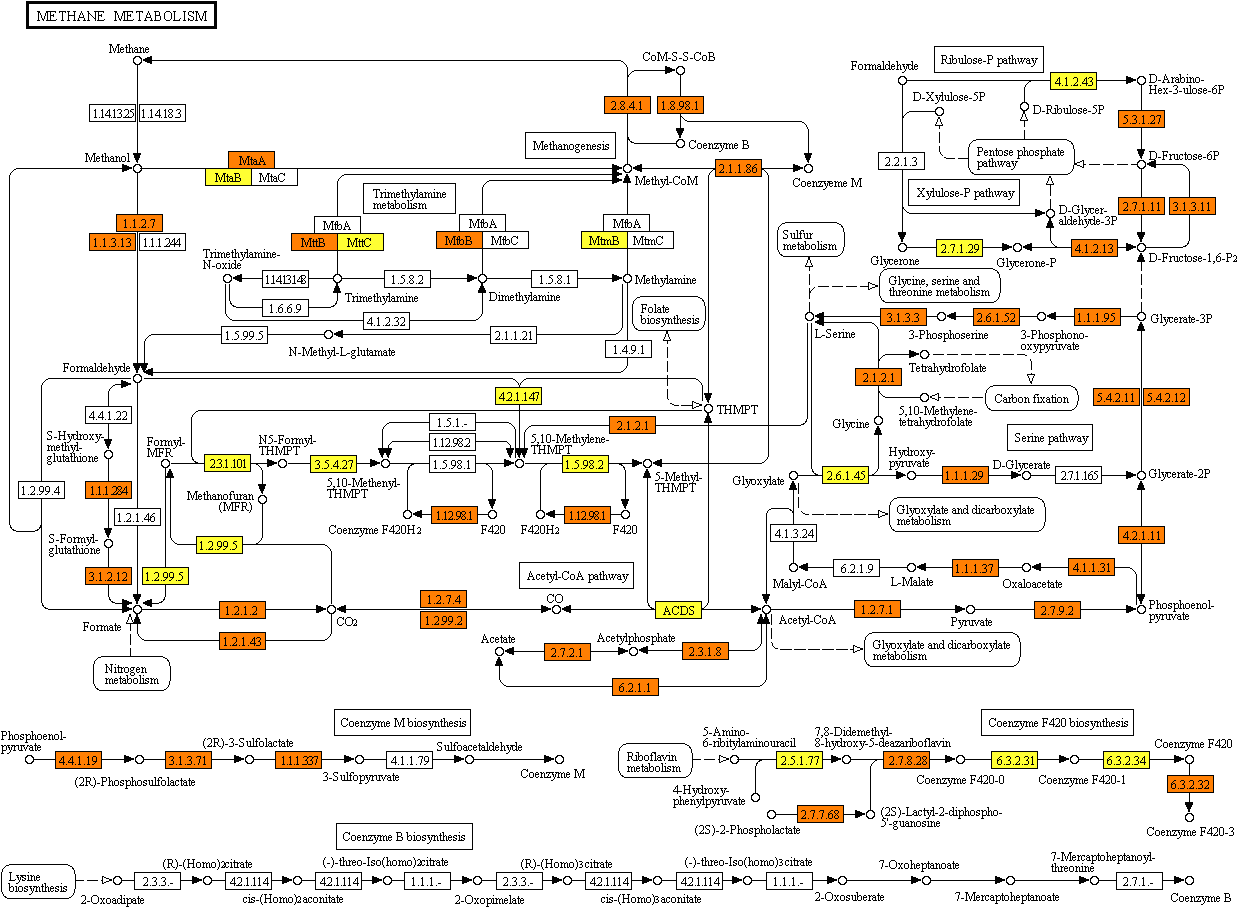
\includegraphics[width=.9\textwidth]{map00680_cropped}
\caption{\csentence{Methane metabolism pathway analysis.} Genes reconstructed in our assembly, that are involved in the methane metabolism [PATH:\href{http://www.genome.jp/kegg-bin/show_pathway?map00680}{map00680}], are highlighted in yellow.
Base pathway image copyrighted by Kanehisa Laboratories.}
\label{fPathway}
\todo[inline]{Nicer (?) alternative: 2 colors, metagenome and metatranscriptome!}
\end{figure}
\begin{figure}[h!]
\centering
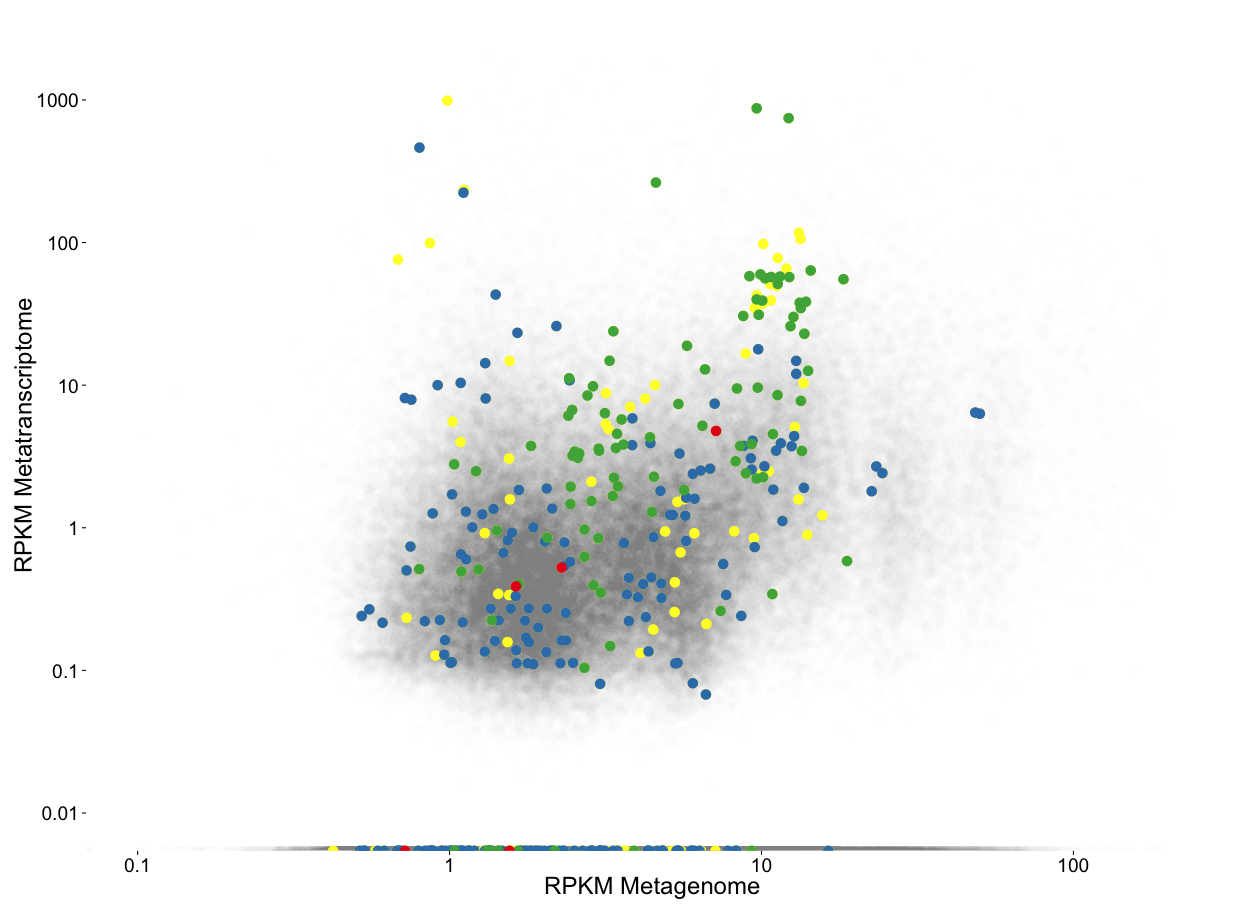
\includegraphics[width=.9\textwidth]{Rplot}
\caption{\csentence{Relating the metagenome and metatranscriptome.} Highlighted are genes involved in methanogenesis, color coded by pathway type: CO2 to methane [MD:\href{http://www.kegg.jp/kegg-bin/show_module?M00567}{M00567}] green, methanol to methane [MD:\href{http://www.kegg.jp/kegg-bin/show_module?M00356}{M00356}] red, and acetate to methane [MD:\href{http://www.kegg.jp/kegg-bin/show_module?M00357}{M00357}] blue.}
\label{fCoverage}
\end{figure}

%%%%%%%%%%%%%%%%%%%%%%%%%%%%%%%%%%%
%%                               %%
%% Tables                        %%
%%                               %%
%%%%%%%%%%%%%%%%%%%%%%%%%%%%%%%%%%%

%% Use of \listoftables is discouraged.
%%

\section*{Tables}
\begin{table}[h!]
\caption{Characteristics of the studied biogas plant. Primary digester, sampling date: Nov 15, 2010.}
\begin{tabular}{rl}
\hline
Process parameter & Sample\\
\hline
Net volume & $2041\,m^{3}$\\
Dimensions & $6.4\,m$ high, diameter of $21\,m$\\
Electrical capacity & $537\,kW_{el}$\\
\hline
pH & $7.83$\\
Temperature & $40\,^{\circ}{\rm C}$\\
Conductivity & $22.10\,mS/cm$\\
Volative organic acids (VOA) & $5327\,mg/l$\\
Total inorganic carbon (TIC) & $14397\,mg/l$\\
VOA/TIC & $0.37$\\
Ammoniacal nitrogen & $2.93\,g/l$\\
Acetic acid & $863\,mg/l$\\
Propionic acid & $76\,mg/l$\\
\hline
Fed substrates & $72\,\%$ maize silage, $28\,\%$ pig manure\\
Organic load & $4.0\,kg\,oDM\,m^{-3}\,d^{-1}$\\
Retention time & $55\,d$\\
Biogas yield & $810.5\,l/kg\,oDM$\\
Methane yield & $417.8\,l/kg\,oDM$\\
\hline
\end{tabular}
\label{tBiogasPlant}
\end{table}

\begin{table}[h!]
\caption{Overview of the different sequencing libraries.}
\begin{tabular}{lllrrrr}
\hline
Accession & Library name & Library type & Insert size$^{1}$ & Cycles & Reads & Bases \\
\hline
ERS697694 & GAIIx, Lane 6 & RNA, TruSeq & $202 \pm 49$ & $2 \times 161$ & $78,752,308$ & $12,679,121,588$ \\
ERS697688 & GAIIx, Lane 7 & DNA, TruSeq & $157 \pm 19$ & $2 \times 161$ & $54,630,090$ & $8,795,444,490$ \\
ERS697689 & GAIIx, Lane 8 & DNA, TruSeq & $298 \pm 32$ & $2 \times 161$ & $74,547,252$ & $12,002,107,572$ \\
ERS697690 & MiSeq, Run A1 & DNA, Nextera & $173 \pm 53$ & $2 \times 155$ & $4,915,698$ & $761,933,190$ \\
ERS697691 & MiSeq, Run A2 & DNA, Nextera$^{2}$ & $522 \pm 88$ & $2 \times 155$ & $1,927,244$ & $298,722,820$ \\
ERS697692 & MiSeq, Run B1 & DNA, Nextera & $249 \pm 30$ & $2 \times 155$ & $3,840,850$ & $573,901,713$ \\
ERS697693 & MiSeq, Run B2 & DNA, Nextera$^{2}$ & $525 \pm 90$ & $2 \times 155$ & $4,114,304$ & $614,787,564$ \\
\hline
\end{tabular}
\label{tReads}
\\$^{1}$Insert sizes determined with Picard tools. $^{2}$This Nextera library was sequenced twice.
\end{table}

\begin{table}[h!]
\caption{Metagenomic and metatranscriptomic sequencing.}
\begin{tabular}{lrrrr}
\hline
Library type & Reads, raw & post-QC & Bases, raw & post-QC\\
\hline
Metagenome (total) & $143,975,438$ & $137,365,053$ & $23,046,897,349$ & $17,267,320,221$ \\
Metatranscriptome & $78,752,308$ & $73,165,986$ & $12,679,121,588$ & $8,455,809,264$ \\
\hline
\end{tabular}
\label{tPostQC}
\end{table}

\begin{table}[h!]
\caption{Metagenome assembly statistics, minimum contig size of $1,000\,bp$.}
\begin{tabular}{rl}
\hline
Assembly metric & Our assembly\\
\hline
Total size & $228,382,457\,bp$\\
Number of contigs & $54,489$\\
N50 value & $9,796\,bp$\\
Largest contig & $333,979\,bp$\\
\hline
Predicted genes & $250,596$\\
of these, full-length & $172,372\,(69\,\%)$\\
Match in KEGG Genes (10) & $241,153$\\
Match in KEGG Genes (1e-3) & $200,214$\\
Match in KEGG Genes (1e-6) & $191,766$\\
Match in KEGG Genes (1e-9) & $184,251$\\
of these, assigned KO & $xxx,xxx$\\
\hline
\end{tabular}
\label{tAssembly}
\todo[inline]{KOs to be added asap, see above.}
\end{table}

%%%%%%%%%%%%%%%%%%%%%%%%%%%%%%%%%%%
%%                               %%
%% Additional Files              %%
%%                               %%
%%%%%%%%%%%%%%%%%%%%%%%%%%%%%%%%%%%

%\section*{Additional Files}
%  \subsection*{Additional file 1 --- Sample additional file title}
%    Additional file descriptions text (including details of how to
%    view the file, if it is in a non-standard format or the file extension).  This might
%    refer to a multi-page table or a figure.
%
%  \subsection*{Additional file 2 --- Sample additional file title}
%    Additional file descriptions text.


\end{backmatter}
\end{document}
